This chapter is a reprint of: \\
Sun, Yang, Martin, Tonegawa. \textit{Nature Neuroscience} \textbf{23}, 1375--1383 (2020). \\
DOI: 10.1038/s41593-020-0681-z

\section*{Abstract}

The brain codes continuous spatial, temporal, and sensory changes in daily experience. Recent studies suggest the brain also tracks experience as segmented subdivisions (events), but the neural basis for encoding events remains unclear. We designed a maze for mice composed of 4 materially indistinguishable lap events, and report hippocampal CA1 neurons whose activity is modulated not only by spatial location, but also lap number. These ``event-specific rate remapping'' (ESR) cells remain lap-specific even when the maze length is unpredictably altered within trials, suggesting ESR cells treat lap events as fundamental units. The activity pattern of ESR cells is reused to represent lap events when the maze geometry is altered from square to circle, suggesting it helps transfer knowledge between experiences. ESR activity is separately manipulable from spatial activity, and may therefore constitute an independent hippocampal code: an ``event code'' dedicated to organizing experience by events as discrete and transferable units.

\section{Introduction}

How is daily experience represented in the brain? Most daily experiences involve travelling to different places and/or seeing different things, and so contain a multitude of spatial and sensory variations. Hippocampal cells monitor these continuous changes in space, passing time, and sensory stimuli\cite{sun2020}.

Meanwhile others, based on recent human imaging studies\cite{sun2020}, have suggested that besides tracking the continuously changing sensory environment, the brain also tracks daily experience as a chain of its discrete, segmented subdivisions or events. Each event arises as a discrete epoch of experience, with its continuous sensory and spatial changes grouped together as a unit. It has been suggested that events are abstract and generalizable entities, and can be divorced from specific sensory details. Take dining in a restaurant as an example. Two different dinner experiences can share the same set of events: eating an appetizer, main course, and dessert, even if they occur at different restaurants, involve different foods, and last varying amounts of time. In other words, each of these events have a degree of invariance to the variations of their actual physical and sensory contents. Instead, these events are defined by the abstract, ordered relationships to one another: an appetizer is eaten first, followed by a main dish, which is followed by dessert. This allows events to describe widely varying experiences in a generalized manner. Encoding these abstract events are important in order to behave perspicaciously in the world.

Beyond representing continuous changes in space, there is evidence that hippocampal neurons encode broader episodic information, including changes in sensory cues as well as past and future trajectories. Hippocampal neurons encode this broader episodic information by changing the activity rate at a given place field (rate remapping). However, neural representations dedicated to encoding events as units of experience, separate from the tracking of the immediate continuous environment, remain poorly understood.

In this study, we have found a hippocampal representation that treats events as discrete units of experience, and we show that these event representations can be transferred between different experiences. We also show that this representation is reciprocally and independently manipulable from the continuous representation of space.

\section{Results}

\subsection{Task design to study segmentation of experience into units}

With oft-used behavioral paradigms that involve changes in spatial and sensory variables, it is difficult to identify neurons tracking discrete and unitary events as opposed to tracking continuous sensory stimuli or spatial differences. For these reasons, we designed a repetitive behavioral task in which sensory cues and spatial trajectories were kept constant for multiple events. This allowed the influence of events as fundamental units to be separated from the influence of changing sensory/spatial information.

In our task, mice repeatedly ran through a square maze subdivided into four laps per trial. A reward was delivered at the onset of lap 1 of every trial, as a single temporal cue, with the subsequent three laps unrewarded. It is known that salient stimuli can potentially serve as boundaries between events. It is possible that reward box visits may serve as event boundaries between lap events. In fact, these mice visited the reward box after every lap, regardless whether a reward was delivered or not. We asked whether there is evidence of neurons that track lap events as discrete units of experience.

A virus expressing the calcium indicator GCaMP6f was injected into dorsal CA1 (dCA1) of the hippocampus in Wfs1 promoter-driven Cre transgenic mice. A microendoscope was implanted above dCA1 to enable long-term calcium imaging in freely moving mice. We recorded calcium activity and characterized the spatial selectivity of CA1 neurons as mice ran the square maze. During testing, animals completed 15--20 trials (60--80 laps) in succession. On average, test mice took 98 seconds to complete one trial. For each neuron during each of the four laps, we calculated its average calcium activity level during moving periods ($> 4$ cm/s) within spatial bins that tiled the maze. In total, 72\% (2509/3506) of CA1 cells from 14 animals were significant place cells. Some neurons were found to be most active during reward consumption (lap 1) in the reward box; these cells were excluded from further analysis because they were active in direct response to the reward. In general, neurons that were active in the start box during non-rewarded laps, or in the maze, were active at the same location on every lap, but showed higher activity for a specific lap compared to other laps.

Since CA1 activity is sensitive to a variety of behavioral variables including spatial location, running speed, and head direction, we fitted the activity of each neuron to a linear model incorporating the animal's spatial location, head direction, and running speed in order to investigate whether these modelled variables were enough to account for the lap preference. We then calculated the remaining calcium activity across four laps that was not accounted for by the model, and referred to this activity as `model corrected', or MC, calcium activity. Each CA1 cell had a lap number during which the cell had the highest activity rate (its preferred lap), and in thirty percent of CA1 cells (1055/3506 cells, $n = 14$ mice), this peak, lap-specific MC activity was significantly different (outside the 95th confidence interval) compared to shuffles. Although CA1 calcium activity exhibited stochasticity in its trial-by-trial activation, these significant lap-modulated CA1 cells exhibited a systematic lap-modulated pattern that was robust across trials. As a control comparison, the percentage of lap-modulated CA1 cells was reduced when reward was given every lap (9\% = 101/1072 cells, $n= 5$ animals). Within the confines of the 4-identical lap task structure, this lap event-specific MC activity is manifested as a sequence of rate remapping over a constant place field location. These cells are henceforth called ``event-specific rate remapping cells'', or ESR cells. All the other CA1 cells were considered non-ESR cells. In order to study the pattern of calcium activity modulated by lap for a given ESR cell, we compiled its lap modulated MC activity in the peak spatial bin for all four laps; we call this sequence of differential activity levels across the four laps the ESR activity pattern. For the rest of this study, we will investigate the features of the experience which give rise to the ESR phenomenon.

For a set of 5 animals that were exposed to the 4-lap-per-trial task for the first time, the percentage of ESR cells was 17\% (176/1008 cells, $n=5$ mice), but following eight days training on the lap task, the proportion rose to 29\% for these same mice (335/1168 cells; $\chi^2 =37.9, p = 7.4 \times 10^{-10}$), showing that ESR activity patterns are learned. Correspondingly, mice did not run at increased speed during the 4th lap compared to the 1st lap during the first exposure to the 4-lap task, but they ran significantly faster during the 4th lap compared to the 1st lap following eight days of training on the 4-lap task. In addition, once mice had been well-trained, if reward was unexpectedly delayed by an extra lap on some trials, mice still ran significantly faster on the 4th lap compared to the 1st lap, but also ran significantly slower during this extra 5th lap compared to the 4th lap, suggesting that animals anticipated reward exactly at the end of the 4th lap.

We tracked ESR cells across days in order to examine the preservation of ESR activity patterns. For every individual ESR cell on day 1, we defined an index for how much the ESR activity patterns are preserved across days as the Pearson correlation of its ESR activity pattern on day 1 vs day 2. The proportion of ESR cells that were highly preserved across days was significantly greater than chance for each of the separate populations of lap 1 cells, lap 2 cells, lap 3 cells, and lap 4 cells. Lap 1, 2, 3 and 4 ESR activity patterns were highly preserved even when half the trials were eliminated, as measured by the ESR correlation index. Generally speaking, lap 1 cells were more highly represented compared to lap 2, 3 and 4 cells, though all four sub-populations of lap-specific cells were significantly preserved in their own right.


\begin{figure}[htbp]
\centering

\includegraphics[width=\textwidth]{figures/ch_sun2020/fig1.jpg}
\caption[Experimental design to study segmentation of experience into units]{\textbf{Experimental design to study segmentation of experience into units.}
(a) Illustration of experience as (top): sequence of continuous, moment-to-moment variations in space, time, and sensory stimuli; (middle): sequence of discrete events as fundamental units of the experience; (bottom): the behavioral task as a skeletal experience stripped of sensory and spatial differences to identify neuronal representations tracking events as fundamental units.
(b) Implantation of microendoscope into dCA1 of Wfs1-Cre mice with AAV2/5-Syn-flex-GCaMP6f-WPRE-SV40 virus.
(c) Top: Coronal section of hippocampus showing aspiration site (white dotted line) and Wfs1+ cells (green), representative of $n=14$ mice. Bottom: $\Delta F/F$ calcium traces of $n=15$ Wfs1+ (pyramidal) cells in CA1 (red = significant transients).
(d) Standard 4-lap-per-trial experiment: reward delivered at start of lap 1 in the reward box, once every 4 laps.
(e) CA1 calcium activity sorted by spatial position and lap number: activity at same place each lap but higher during a specific lap (263 cells from example animal).
(f) Trial-by-trial calcium activity of example lap 1, 2, 3, and 4 preferring neurons.
(g) Model correction of lap-dependent neuronal activity: raw calcium activity (left) vs.\ model-corrected (MC) calcium activity after subtracting speed- and head-direction-explained variance (right).
(h) Percentage of ESR cells tuned to each lap in the standard 4-lap experiment ($n=14$ animals).
(i--k) Control: reward every lap reduces ESR cell percentage (101/1072 cells vs.\ 371/1328 in standard task; $\chi^2=128.7$, $p < 10^{-16}$, $n=5$ mice).}
\label{fig:sun2020-fig1}
\end{figure}
\subsection{ESR treats events as fundamental units of the experience}

Several key results support the notion that ESR tracks lap events as discrete units of the experience, separate from the continuous moments which also make up the experience. Since previous studies showed that the hippocampus encodes continuously changing variables, we investigated the relationship between ESR activity and several continuous episodic variables more closely. Instead of tracking lap events, could ESR cells be tracking a particular duration of time since the start of the trial? Time cells require a reliable temporal delay period; otherwise they do not arise. Because the animals in our task were allowed to behave freely, and took unpredictable and variable durations to complete the trials of the task and ran at varying speeds, ESR cells were unlikely to act as time cells in our task. Could ESR cells instead be representing the total distance continually travelled along the course of the 4-lap task since the start of the trial? When we elongated the maze in one dimension to twice the usual length, the ESR activity patterns were still significantly preserved across days, suggesting it unlikely that ESR cells directly track the continuous distance traveled.

We conducted another experiment to investigate whether laps are treated as units of experience. A 4-lap-per-trial task was conducted in which the maze was elongated on pseudo-randomly chosen laps of pseudo-randomly chosen trials. Importantly, this maze was largely stripped of predictability in travelled distance but the 4-discrete lap structure was still preserved. A total of 27\% of CA1 cells (306/1128 cells, $n = 6$ animals) active in all trial types of this experiment were significant ESR cells. For these cells, their ESR activity pattern during the standard (short SSSS) trials was still preserved during each of the pseudo-randomly elongated trial types. Thus, ESR activity of this sizeable population of CA1 cells was unperturbed by arbitrary and unpredicted variations within the relevant lap event or even variations within neighboring (preceding and succeeding) lap events. For these cells, their ESR activity was preserved even during SSLL trials compared to LLSS trials, which were trials that had the same total distance but had different internal segmentation into long and short laps. Therefore, ESR activity treats these lap events as separate units of the experience, unaffected by spatiotemporal variations within the current or neighboring event units.


\begin{figure}[htbp]
\centering

\includegraphics[width=\textwidth]{figures/ch_sun2020/fig2.jpg}
\caption[Lap 1, 2, 3, and 4 ESR cells are reliably preserved across days]{\textbf{Lap 1, 2, 3, and 4 ESR cells are reliably preserved across days.}
(a--c) Trial-by-trial (a) and trial-averaged calcium activity of example lap 1, 2, 3, and 4 preferring neurons matched across 2 consecutive days, with (b) spatial activity and (c) ESR activity (MC calcium activity) calculated for each neuron.
(d) Individual ESR cells' calcium activity sorted by spatial location during day 1, with cell order matched across days, confirming preserved place fields (622 cells, $n=8$ animals).
(e) Pearson correlation of ESR activity across days for individual cells (orange: real; grey: shuffled). The proportion with highly preserved ESR patterns (Pearson's $r > 0.6$) was significantly greater than shuffles (622 cells total).
(f) Individual cells show both high ESR correlations and high spatial correlations across days (622 cells).}
\label{fig:sun2020-fig2}
\end{figure}
\subsection{ESR activity is transferrable between experiences}

The results thus far suggest that the lap events being tracked by ESR have a generalizable nature, robust against continuous variabilities like time or distance. If this notion is correct, then we predict that ESR activity should exhibit a degree of independence from sensory and spatial content. To test this concept further, we conducted a two day experiment with the 4-lap-per-reward task on two geometrically distinct mazes. The standard square maze was used on the first day, and a circular maze was used on the second day. Spatial activity of ESR cells globally remapped on the circular maze compared to the standard square maze, as a result of the different geometry of the maze. Nevertheless, a significant proportion of ESR cells tracked circular laps using the same lap-specific activity pattern as the corresponding square maze laps (176/461 total cells = 38\% with ESR correlation $> 0.6$ across days). Thus the knowledge of lap-specificity acquired during the square maze was reused (transferred) when the animals were faced with the circular maze.

To further test the generalizable nature of these lap events, we modified the repetitive square maze by adding spatial trajectory variation. A two-day experiment was conducted in which the 4-lap-per-reward was preserved on the 2nd day, whereas the spatial trajectories were altered every two laps. Here, a significant proportion of lap 1--4 ESR cells still had preserved ESR activity across sessions, coding laps 1--4, despite the animals' experiencing differential spatial trajectories on different laps.


\begin{figure}[htbp]
\centering

\includegraphics[width=\textwidth]{figures/ch_sun2020/fig3.jpg}
\caption[ESR treats events as fundamental units of experience]{\textbf{ESR treats events as fundamental units of experience.}
(a) Left: Four trial types in the random maze elongation experiment (SSSS, LLSS, SSLL, LLLL). Right: Example lap 2 cell ESR and spatial activity across all trial types.
(b) Pseudorandom experiment schedule: 28 trials total, 7 per trial type.
(c--f) ESR correlations of individual cells (306 cells, $n=6$ mice) comparing SSSS vs.\ LLSS (c), SSSS vs.\ SSLL (d), SSSS vs.\ LLLL (e), and SSLL vs.\ LLSS (f). The proportion with highly preserved ESR patterns (Pearson's $r > 0.6$) was significantly greater than shuffles in all comparisons.}
\label{fig:sun2020-fig3}
\end{figure}
\subsection{ESR tracks the relationships between events}

The ESR does not reflect precise sensory information per se, so we hypothesized that it might instead reflect more generalized information from the structure of the task, such as the ordered relationships between the event units. This was suggested by the fact that the 4 lap events of our task are identical to one another in their sensory and spatial content, and yet, ESR activity still reliably distinguished each of the 4 lap numbers (lap 1, 2, 3, 4).

To further test the hypothesis that ESR tracks the ordered relationships between events, we conducted two experiments. First, we conducted an experiment in which the relationships between lap events were abolished. The standard 4-lap-per-trial experiment was conducted on the first day, but the once-in-four lap delivery of the reward (which serves as a temporal marker) was perturbed on the second day and instead the reward was provided every lap. We found that lap 1, 2, 3 and 4 ESR activity pattern preservation was significantly abolished across days.

Second, we conducted an experiment in which the relationships between the lap events were more subtly perturbed, and asked how this affects ESR activity. The standard 4-lap-per-trial experiment was conducted on the first day and a non-rewarded 5th lap was added to all the trials on the second day before reward eating. On day 2, lap 1 and 2 cells had preserved ESR activity despite the added lap. On the other hand, lap 3 cells were abruptly and discretely perturbed. Indeed, a significant portion of lap 3 cells shifted to track lap 4 (17/55 cells = 31\%, $n = 4$ mice). In contrast, only 5/55 cells (= 9\%) maintained their lap 3 preference.

Similarly, lap 4 cells shifted to track lap 5. Although, overall, the pattern of most lap 4 cell activity across the two days was well correlated, a significant proportion of lap 4 cells (42/60 cells = 70\%, $n = 4$ mice, $p < 10^{-4}$ compared to shuffling) showed a significant decrease in overall activity level during lap 4 on day 2 but also showed an apparent, concomitant restoration of activity level during lap 5. This decrease in activity during lap 4, and shift in activity by precisely one lap unit reflects the fact that the 4th lap is no longer rewarded, and that an extra lap is needed to fulfill the total requirement of 5 laps to receive reward. In contrast, only 2/60 cells (= 3\%) maintained their lap 4 preference. Therefore, ESR track the skeletal structure of experience: it tracks events as fundamental units, and the ordered relationships between them.


\begin{figure}[htbp]
\centering

\includegraphics[width=\textwidth]{figures/ch_sun2020/fig4.jpg}
\caption[ESR tracks lap events despite change in maze geometry]{\textbf{ESR tracks lap events despite change in maze geometry.}
(a) Circular maze experiment: Day 1 on standard square maze, Day 2 on circular maze.
(b--d) Example lap 1, 2, 3, and 4 preferring neurons with trial-by-trial calcium activity, spatial activity, and ESR activity matched across square and circular maze sessions.
(e) Individual ESR cells' calcium activity sorted by spatial location on the square track (day 1), cell order matched across days (461 cells, $n=5$ mice).
(f) ESR correlations during square vs.\ circular maze sessions. The proportion with highly preserved patterns (Pearson's $r > 0.6$) was significantly greater than shuffles (461 cells).
(g) Top: Individual cells showed high ESR correlations while spatial fields remapped (461 cells). Bottom: Same for the subpopulation of highly preserved ESR cells: spatial activity was also remapped (176 cells).}
\label{fig:sun2020-fig4}
\end{figure}
\subsection{ESR activity and spatial activity are jointly but separately represented in the same cells}

ESR activity and spatial activity occur jointly in the same cells. But what is the relationship between these two representations? Within the confines of the standard 4-lap task, ESR activity is manifested as the differential activity rate during each of the different laps at the same spatial field location, and is therefore a form of rate remapping. We then investigated whether this ESR activity pattern is necessarily tied to its particular place field location by testing whether ESR activity could be reciprocally and separately manipulable from the spatial activity.

When the maze and task were not altered in any way across days, both ESR activity patterns and spatial activity patterns remained unperturbed. In contrast, as we previously showed, the 4-lap task conducted on a circular maze geometry distorted the spatial activity but ESR activity remained largely intact, showing that ESR activity is not tied to its particular place field location. Can the converse result, an alteration of ESR activity pattern without concomitant alteration of the spatial activity pattern, be observed? First, perturbing the relationships between events by adding a lap altered some ESR activity patterns but spatial activity was still preserved in the same cells. Second, we investigated MEC axonal terminal inhibition in CA1 and asked how it affects the ESR activity versus the spatial activity patterns. Medial entorhinal cortex (MEC) input into hippocampus has been implicated in the sequential organization of experiences, although this is not the only brain region to be so implicated. Based on these earlier studies, a virus expressing inhibitory opsin was injected bilaterally into the MEC sub-region of pOxr1-Cre mice. In addition, a virus expressing the calcium indicator GCaMP6f was unilaterally injected into dorsal CA1 (dCA1) of the same mice. An opto-endoscope was implanted above dCA1 to enable long-term calcium imaging as well as optogenetic inhibition of the axonal terminals from MEC neurons in dCA1. The mice ran 28--40 trials of the 4-lap task where the trials alternated between optogenetic inactivation (Light-On) and no inactivation (Light-Off) of the MEC axonal terminals. Inactivation of MEC terminals in dCA1 did not change the spatial activity patterns in dCA1, consistent with previous studies. And yet, this inactivation altered ESR activity patterns in the same cells. By contrast, control mice that were injected with control virus had preserved ESR activity patterns across Light-On and Light Off trials.

Taken together, the lap-specific activity pattern (ESR) is reciprocally and independently manipulable from spatial activity, although the two representations are expressed jointly in the same cells.


\begin{figure}[htbp]
\centering
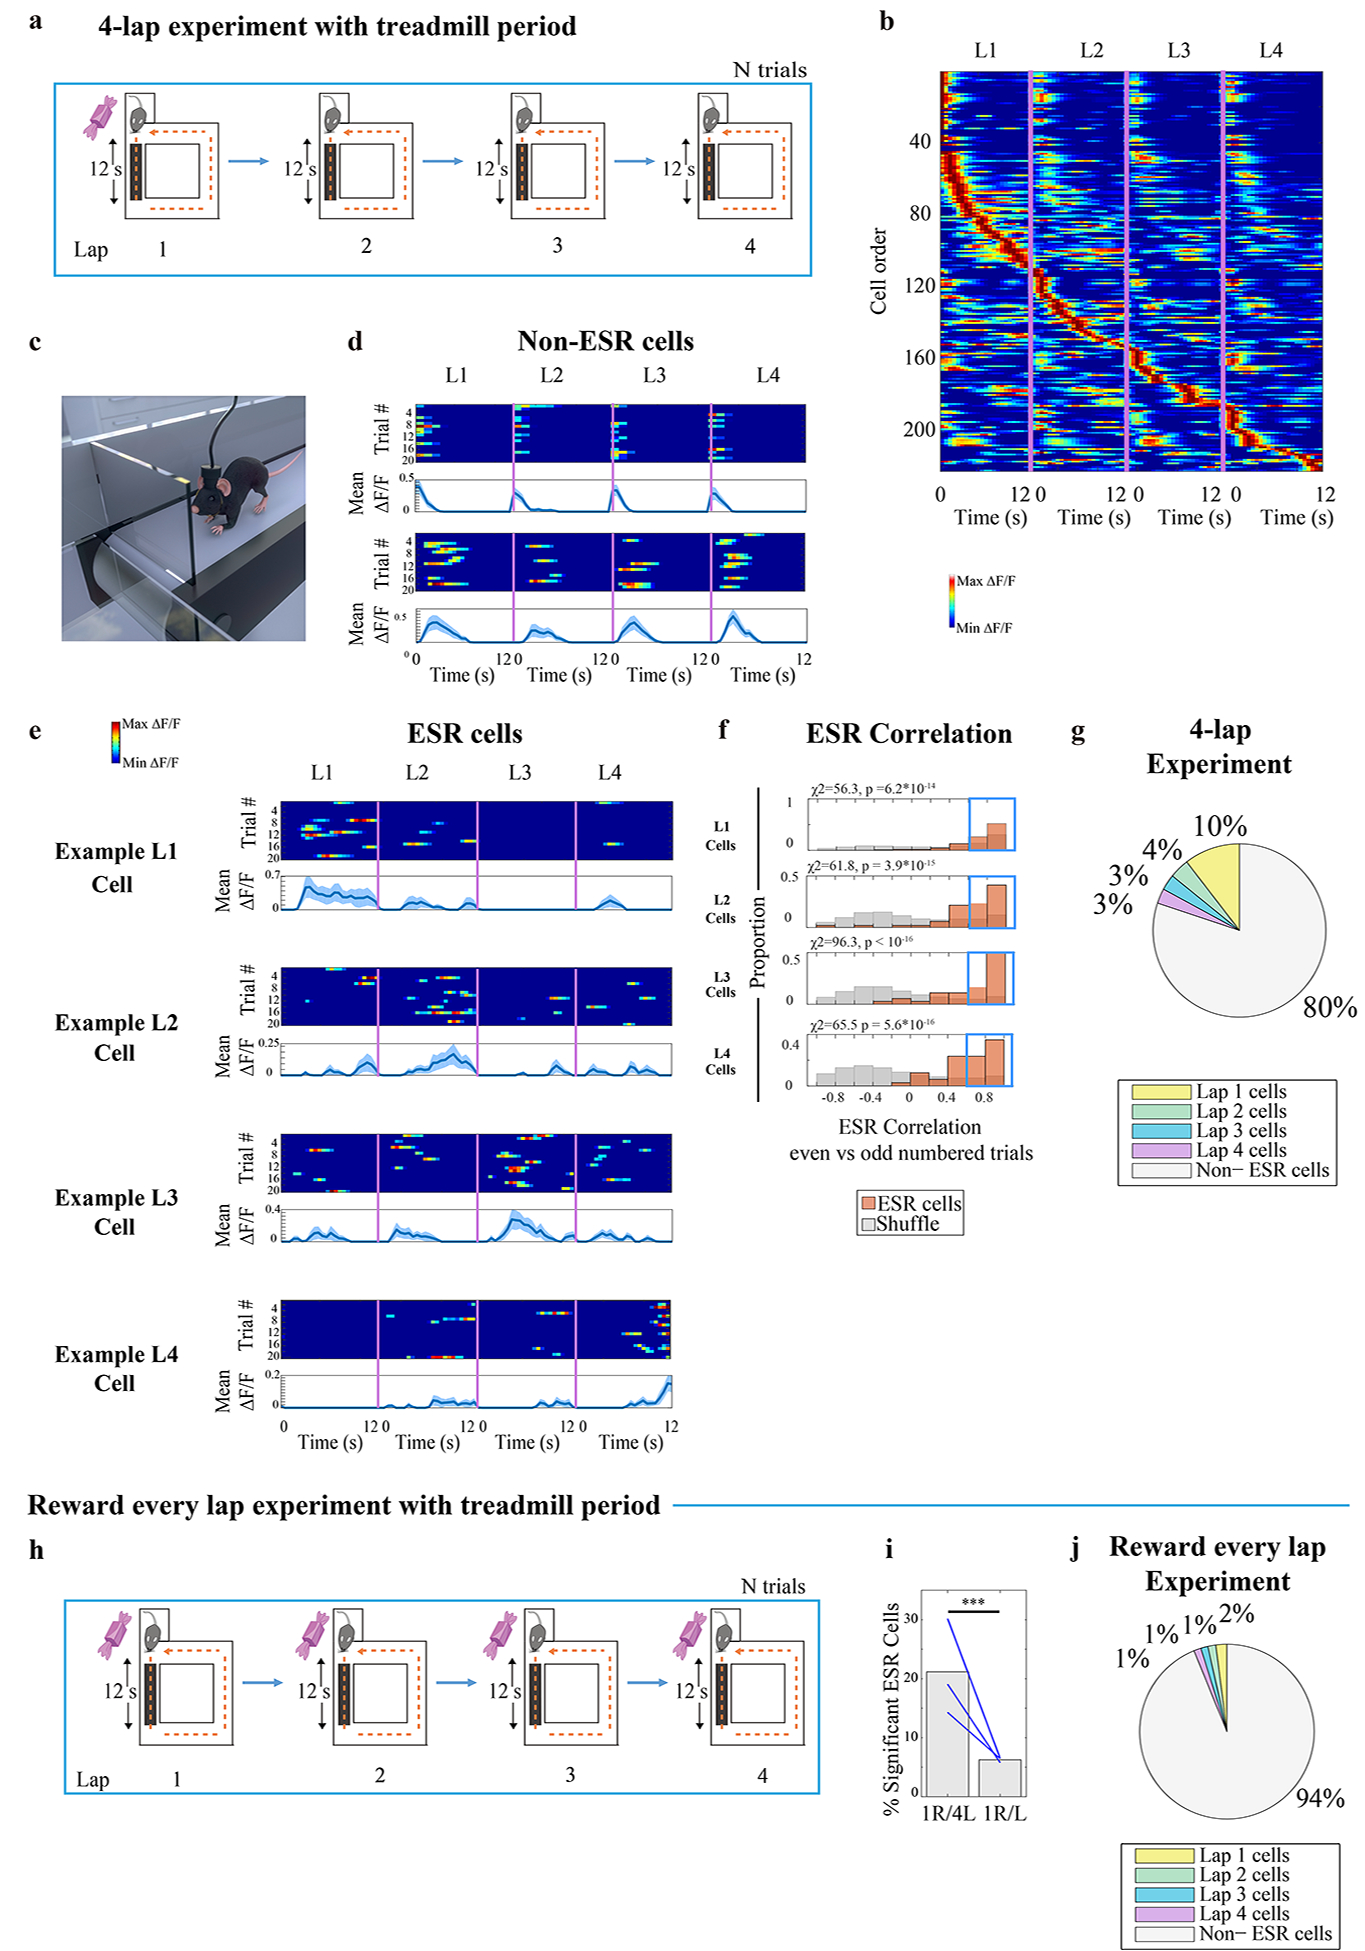
\includegraphics[width=\textwidth]{figures/ch_sun2020/fig5.jpg}
\caption[ESR tracks the relationships between events]{\textbf{ESR tracks the relationships between events.}
(a--c) Reward-every-lap experiment: ESR correlations (134 cells, $n=3$ mice) showing perturbation of ESR but preservation of spatial activity when event relationships are abolished.
(d) Lap addition experiment: Day 1 standard 4-lap-per-trial; Day 2 with 5-lap-per-trial.
(e) ESR correlations across 4-lap and 5-lap sessions (382 cells, $n=4$ mice).
(f) Lap 3 cells: high spatial correlation but perturbed ESR in the lap addition experiment (55 cells).
(g) Two example neurons transformed from lap 3 to lap 4 preference.
(h) Percentage of cells transformed from lap 3 to lap 4 (17/55, $n=4$ mice).
(i) Two example neurons transformed from lap 4 to lap 5 preference.
(j) Percentage of cells transformed from lap 4 to lap 5 (42/60, $n=4$ mice).
(k) MC activity of lap 4 cells significantly decreased during lap 4 on day 2 ($z=4.57$, $p=4.88 \times 10^{-6}$).
(l) MC activity of lap 4 cells was not significantly different from lap 5 activity on day 2 ($z=-0.72$, $p=0.47$).}
\label{fig:sun2020-fig5}
\end{figure}
\subsection{Discrete event modulated activity occurs together with continuous non-spatial activity}

ESR activity and spatial activity are jointly represented in the same cells. What happens when the main continuous changes in the experience are not spatial? To answer this question, we conducted another 4-lap-per-trial experiment in which the first arm of the standard 4-lap-per-trial maze was replaced by a treadmill. Animals ran for 12 s on the treadmill at 14 cm/s on every lap. Monitoring activity of neurons on a treadmill obviates the necessity of model corrections for running speed and head direction changes because they are nearly constant on the treadmill. Consistent with previous studies, cells are active during this non-spatial treadmill period. During the period restricted to the treadmill, 20\% of CA1 cells (243/1222 cells, $n = 5$ animals) had significantly lap-modulated activity, which exhibited a systematic lap-modulated pattern that was robust across trials. The percentage of ESR cells was reduced when reward was given every lap (6\% = 42/681 cells, $n = 3$ animals). These results indicate that the tracking of experiences by the hippocampus occurs a joint manner with an event-specific representation along with a continuous variable-tracking representation, even when the continuous experience is primarily non-spatial in nature.


\begin{figure}[htbp]
\centering
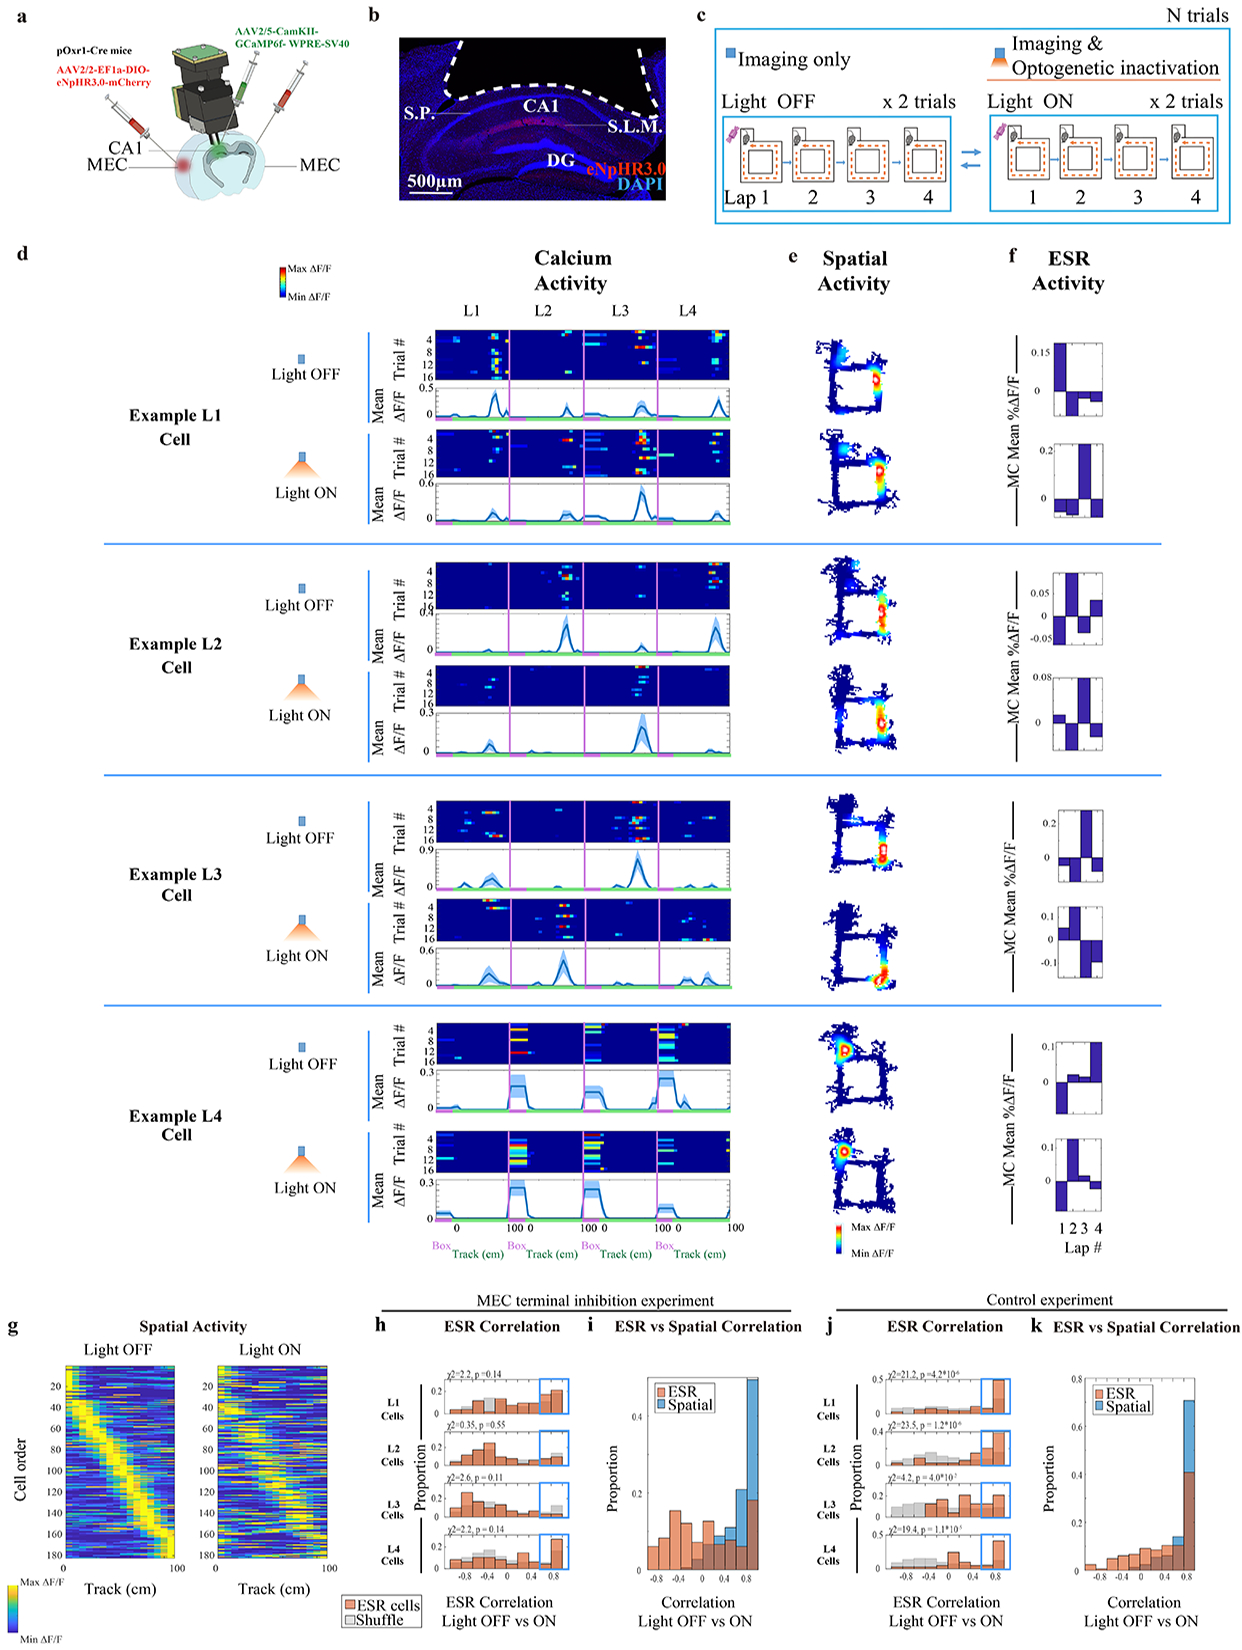
\includegraphics[width=\textwidth]{figures/ch_sun2020/fig6.jpg}
\caption[ESR activity and spatial activity are separately manipulable]{\textbf{ESR activity and spatial activity are separately manipulable.}
(a) Simultaneous CA1 imaging and MEC terminal inhibition in CA1.
(b) Coronal section showing aspiration site and MEC inputs (eNpHR3.0, red). S.L.M.\ = stratum lacunosum moleculare; S.P.\ = stratum pyramidale. Representative of $n=6$ pOxr1-Cre mice.
(c) Optogenetics light-On and light-Off conditions alternated every 2 trials (32--40 trials total).
(d--f) Example lap 1, 2, 3, and 4 preferring neurons matched across light-Off vs.\ light-On trials.
(g) Individual ESR cells' calcium activity sorted by spatial location, cell order matched across conditions (182 ESR cells, $n=3$ mice).
(h) ESR correlations across light-On vs.\ light-Off: the proportion with preserved ESR patterns was not significantly greater than shuffles (182 cells).
(i) Individual cells showed high spatial correlations while ESR representations were perturbed (182 cells).
(j) ESR correlations for control mice (AAV2/2-EF1a-DIO-mCherry; 164 ESR cells, $n=3$ mice).
(k) Control mice showed both high spatial and ESR correlations across light-On vs.\ light-Off (164 cells).}
\label{fig:sun2020-fig6}
\end{figure}
\section{Discussion}

\subsection{ESR tracks discrete units of experience}

While mice ran a 4-lap-per-reward task, approximately 30\% of individual CA1 pyramidal neurons exhibited calcium activity levels that were significantly higher during one of the four laps. This ESR activity tracked the identities of laps despite variations in time duration needed to cover the lap events and even when pseudorandom variations in distance travelled were introduced during lap events. Therefore, ESR activity treats lap events as separate event units that are unaffected by spatiotemporal variations within current or neighboring events. In CA1 pyramidal cells, the ESR activity and spatial activity are jointly represented, so CA1 cells are active at a particular spatial field on the maze, at a differential activity rate. But ESR activity tracks the lap identity even when this CA1 cell's spatial field was moved to an arbitrary location on a different maze. Taken together, this shows that ESR treats different locations of a particular lap as part of the same event unit. When ESR was changed, it changed as a discrete, lap-specific shift---rather than gradually through the course of the task experience.

Our finding of the ESR phenomenon is consistent with the theoretically derived concept and data obtained by human imaging studies that alongside codes tracking continuous changes in spatial and sensory content, the brain tracks an experience by identifying one discrete, unitary event after another, as the entire experience progresses. These previous studies showed the brain's involvement in event segmentation by showing heightened Blood Oxygen Level Dependent (BOLD) activity at the boundaries between events, an observation that was recently confirmed by electrophysiology. Our present study provides further insight into the encoding of events by identifying a representation within single cells (ESR activity) that is tuned to the event units themselves, rather than solely the event boundaries. ESR activity treats these events as fundamental units that make up the experience, and could therefore be part of the neurophysiological basis for encoding events by the brain.

\subsection{ESR tracks abstract, relational features of events and could support ``transfer learning''}

Recent human imaging and computational studies, including a computational model termed the ``Eichenbaum-Tolman machine'', have suggested that the hippocampus is involved in coding the abstract structure which composes an episodic experience. Consistent with these studies, our present work, at the single cell level, suggests a hippocampal activity pattern (ESR) that not only tracks events, it tracks these events as putatively abstract entities. Indeed, our results show that the ESR consistently tracked lap events, irrespective of concrete sensory and spatiotemporal variations within the events. Furthermore, ESR tracks the abstract and iterative relationships between events. In fact, we show that ESR activity reliably distinguishes the 4 lap events which are materially identical to one another but differ in their iterative and ordered relationships to the preceding and succeeding lap numbers. Could the ESR differentially represent the 4 laps simply because it represents an internal variable like the gradually increasing level of motivation for acquiring another reward? This is unlikely for two reasons. First, ESR activity patterns are not affected by arbitrary variations in the time and travelled distance required to complete the trial and receive reward. Even during LLLL trials, which were presented to the animal in an unpredictable fashion and where the animal had to run on a maze length that was twice as long as the standard maze in order to reach reward, ESR activity patterns remained lap specific. Second, when an additional 5th lap was added to every trial in the task, lap 3 and 4 cells changed their activity on their respective lap, and shifted their activity by precisely one lap unit. This result suggests that ESR cells differentiate between the lap numbers as the animal's running progresses, and reflects the precise knowledge that lap number 4 is no longer rewarded, and that a 5th counted lap is now necessary to receive reward. Altogether, our results indicate that ESR tracks the skeletal structure of experience via events as abstract entities, with abstract relationships between them.

In real life there are few truly novel experiences: most new experiences share either physical or abstract features with past experiences. Learning a new task is improved through the transfer of knowledge from the web of related tasks that have already been learned, a phenomenon called ``transfer learning''. ESR appears to track the events as abstract units and their abstract relationships, and may therefore facilitate the transfer of knowledge between experiences that share these abstract features even if concrete spatial and sensory stimuli are distinct. Indeed, when the geometry of the maze was shifted from square to circular under the 4 laps per reward conditions, ESR activity was significantly maintained across these different experiences even though place field activity was globally remapped. ESR activity could therefore capture not only the abstract structure within an experience, but also provides the elements (events) that can be reused during a different experience.

\subsection{ESR activity is independently manipulable from continuous spatial activity}

Previous studies demonstrated that hippocampal cells change their firing rate in a particular spatial field in response to broader experiential changes, including sensory cues and past and future trajectory changes. This has been termed rate remapping. Consistent with these studies, ESR also showed up as a pattern of rate remapping within the confines of the standard 4-lap task.

Yet, ESR activity possesses an additional property: the pattern of rate remapping (i.e.\ ESR activity) is maintained, even when the place field location is moved to a new spatial location. These data indicate that ESR is not tied to a particular place field location. In a reciprocal manner, ESR activity patterns could also be perturbed without a concomitant perturbation of spatial activity patterns, for instance by the addition of a lap into the task and also by optogenetically inhibiting incoming MEC fibers. ESR activity's influence on neuronal activity is therefore mechanistically separate from the spatial activity's influence. Together, these results demonstrate that ESR activity is reciprocally and independently manipulable from spatial activity, without affecting each other.

What are the benefits of tracking experience in a joint manner with both discrete and continuous representations? In fact, the two neural representations track different aspects of the same episodic experience. The tracking of immediate experience within an event likely requires a level of detail that would be best served by a continuous (spatial or non-spatial) neural representation. On the other hand, tracking extended experience in a compact, flexible, and generalizable way likely requires a level of abstraction above the moment to moment variational details and may be best served by encoding discrete and abstract event units. Ultimately, we found that ESR activity tracks events as fundamental units, is transferable between different experiences, and is independently manipulable from continuous spatial activity. We propose that it might therefore constitute an independent code from the spatial code: an ``event code'' that is dedicated to tracking events as discrete units of experience, alongside codes monitoring continuously changing variables. This event code may help the brain track experience in an efficient and flexible manner.


\begin{figure}[htbp]
\centering
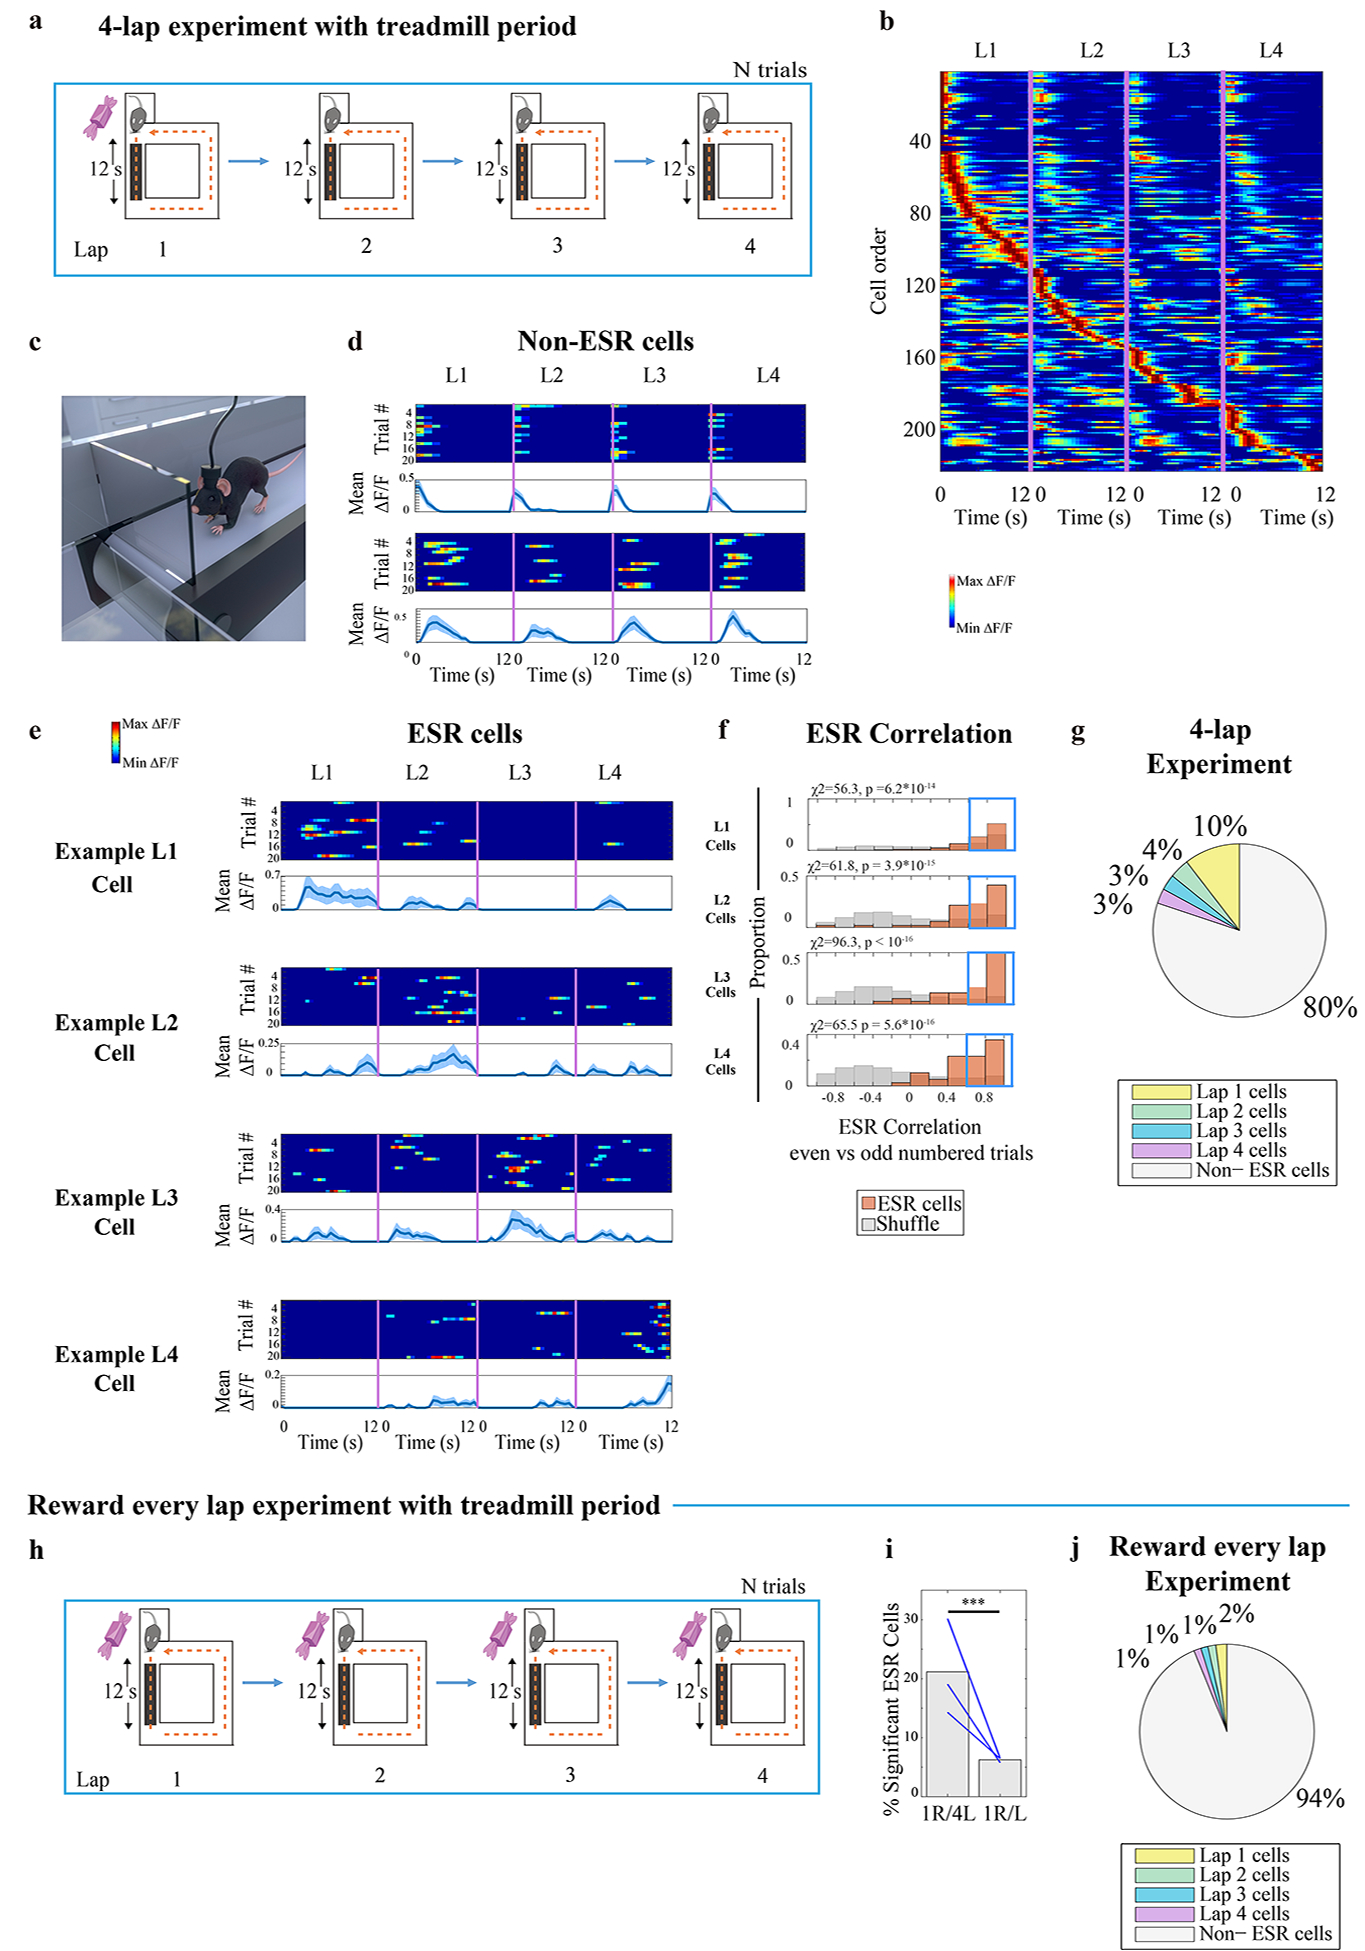
\includegraphics[width=\textwidth]{figures/ch_sun2020/fig7.jpg}
\caption[Discrete ESR activity occurs together with continuous non-spatial activity]{\textbf{Discrete ESR activity occurs together with continuous non-spatial activity.}
(a) 4-lap-per-trial experiment with a 12\,s treadmill period per lap.
(b) CA1 calcium activity sorted by time on the treadmill and lap number, showing activity at the same time each lap but higher during a specific lap (222 cells from example animal).
(c) Cartoon of mouse running during the treadmill period.
(d--e) Trial-by-trial calcium activity of (d) example non-lap-preferring neurons and (e) example lap 1, 2, 3, and 4 preferring neurons during the treadmill period.
(f) ESR correlations between even- and odd-numbered trials for individual ESR cells (243 cells, $n=5$ mice): the proportion with highly preserved patterns (Pearson's $r > 0.6$) was significantly greater than shuffles.
(g) Percentage of ESR cells tuned to each lap in the 4-lap treadmill experiment (1222 cells, $n=5$ mice).
(h--j) Control (reward every lap): significantly fewer ESR cells during treadmill period ($\chi^2=65.0$, $p=7.8 \times 10^{-16}$, $n=3$ mice).}
\label{fig:sun2020-fig7}
\end{figure}
\section{Methods}

\subsection{Animals}

All procedures relating to mouse care and treatment conformed to the Massachusetts Institute of Technology (MIT)'s Committee on Animal Care guidelines and NIH guidelines. Animals were individually housed in a 12 hour light (7 pm--7 am)/dark cycle. Twenty four male Wfs1-Cre mice aged between 2--4 months were implanted with Inscopix microendoscope into CA1 and food restricted to 85--90\% normal body weight for the experiments. For each of the six main maze manipulation imaging experiments (random maze elongation experiment, circular maze experiment, lap addition experiment, treadmill experiment, fixed maze elongation experiment, spatial alternation experiment) the number of animals used (at least 4) is indicated in the main text for each experiment. In each of these experiments, at least two of these tested animals did not previously undergo any of the other manipulative experiments. The other animals were experienced animals from the other manipulative experiments. Significant ESR cells were found during each of these maze manipulation sessions. Six pOxr1-Cre mice (3 for the MEC terminal inhibition experiment and 3 control mice), aged 2--4 months, were also implanted with Inscopix microendoscope into CA1 for dual imaging and optogenetics experiments, and trained in a same manner as Wfs1-Cre mice.

\subsection{Histology and Immunohistochemistry}

Mice were transcardially perfused with 4\% paraformaldehyde (PFA) in phosphate buffered saline (PBS). Brains were then post-fixed with the same solution for 24 hours, and brains were sectioned by using a vibratome. Sections were stained by DAPI. Micrographs were obtained using a Zeiss AxioImager M2 confocal microscope using Zeiss ZEN (black edition) software.

\subsection{Preparation of Adeno-Associated Virus (AAV)}

The AAV2/5-Syn-flex-GCaMP6f-WPRE-SV40 was generated by and acquired from the University of Pennsylvania Vector Core, with a titer of $1.3 \times 10^{13}$ genome copy/ml. The AAV2/5-CamKII-GCaMP6f-WPRE-SV40 was generated by and acquired from the University of Pennsylvania Vector Core, with a titer of $2.3 \times 10^{13}$ genome copy/ml. The AAV2/2-EF1a-DIO-eNpHR3.0-mCherry was generated by and acquired from the University of North Carolina (Chapel Hill) Vector Core, with a titer of $5.3 \times 10^{12}$ genome copy/ml.

\subsection{Stereotaxic Surgery}

Stereotactic viral injections and microendoscope implantations were all performed in accordance with Massachusetts Institute of Technology (MIT)'s Committee on Animal Care guidelines. Mice were anaesthetized using 500 mg/kg avertin. Viruses were injected by using a glass micropipette attached to a 10 $\mu$l Hamilton microsyringe through a microelectrode holder filled with mineral oil. A microsyringe pump and its controller were used to control the speed of the injection. The needle was slowly lowered to the target site and remained for 10 minutes after the injection.

For CA1 imaging experiments, unilateral viral delivery into the right CA1 of the Wfs1-Cre mice was aimed at coordinates relative to Bregma: AP: $-2.0$ mm, ML: $+1.4$ mm, DV: $-1.55$ mm. Wfs1-Cre mice were injected with 300 nl of AAV2/5-Syn-flex-GCaMP6f-WPRE-SV40. Approximately one month after injection, a microendoscope was implanted into the dorsal part of CA1 of the Wfs1-Cre mice aimed at coordinates relative to Bregma, at: AP: $-2.0$ mm, ML: $+2.0$ mm, and DV at approximately $-1.0$ mm. To implant at the correct depth, the cortex was vacuum-aspirated which resulted in the removal of corpus callosum, which is visible under surgery microscope as fibers running in the medial-lateral direction. The fibers of the alveus, which are visible as fibers running in the anterior-posterior direction, were left intact by the procedure.

For CA1 optogenetic and imaging experiments, 300 nL (AAV2/5-CamKII-GCaMP6f-WPRE-SV40) unilateral viral delivery into the right CA1 of the pOxr1-Cre mice was aimed at coordinates relative to Bregma: AP: $-2.0$ mm, ML: $+1.4$ mm, DV: $-1.55$ mm, and 300 nL (AAV2/2-EF1a-DIO-eNpHR3.0-mCherry) bilateral viral delivery into the MEC of these mice were aimed at coordinates relative to Bregma: AP: $-4.85$ mm, ML: $\pm 3.45$ mm, DV: $-3.35$ mm. Control pOxr1-Cre mice received the same CA1 viral delivery, and also received a bilateral delivery into MEC, but the bilaterally delivered virus was the control virus AAV2/2-EF1a-DIO-mCherry. Following these virus injections, the micro-endoscopy lens was implanted in the same manner for these dual optogenetic and imaging experiments, as described above for CA1 imaging experiments.

The baseplate for miniaturized microscope camera was attached above the implanted microendoscope in the mice. After experiments, animals were perfused, and post hoc analyses were examined to determine actual imaging position in CA1.

\subsection{Apparatus Description and Experimental Conditions}

The apparatus was a square maze 25 cm in length and width, with a 5 cm wide track width, and 7 cm height. A 10 cm $\times$ 10 cm square reward box was located in one corner of the square maze. Sugar pellets were placed in the reward box at the beginning of lap 1 of each trial. Four versions of this apparatus were used. Version 1 was used in the standard 4-lap-per-trial experiments. Version 2 used in the random maze elongation experiment had a length elongation to twice the standard length (50 cm = 2 $\times$ 25 cm), but was otherwise identical to Version 1 in other dimensions. Version 3, used in the treadmill experiment, had a 18 cm long treadmill installed in the arm of the maze that immediately faces the reward box. Version 3 otherwise used the same dimensions as Version 1. Version 4, used in the spatial alternation experiment, had an 8-maze configuration, with the other square of the 8-maze being 25 cm in length and width as well. Version 4 otherwise used the same dimensions as Version 1. The circular maze used in the circular maze experiment was constructed to have the same total path length (i.e.\ circumference) as the Version 1 square maze, as well as the same reward box size. All mazes were opaque and black.

All maze experiments were done under dim light conditions, with prominent visual cues within 50 cm on all sides of the box. Ca$^{2+}$ imaging in the maze lasted at least 20 minutes in order to collect a sufficient number of Ca$^{2+}$ transients to power the statistical analyses. The maze surface was cleaned between sessions with 70\% ethanol. Immediately before and after imaging sessions, the mouse rested on a pedestal next to the maze.

The basic task in this manuscript is the standard 4-lap-per-trial task, where animals traversed round a square maze 25 cm in length (1 m journey in total). The task was designed so that a sugar pellet reward was delivered manually to the reward box, at the beginning of lap 1, once every 4 such laps, which we call a single `trial'. Identical motions were made on each lap, regardless whether a pellet was delivered or not. During the testing, animals completed 15--20 of such trials in repetitive succession without interruption. For any behavioral session in which the animal missed going into the reward box more than once in the entire sequence of runs (15 to 20 $\times$ 4 = 60 to 80 runs in total), the experiment was excluded. Crucially, for all experiments, animals first underwent task training before the final testing days. Training procedures are described below.

\subsection{Task-Specific Training}

Each of the main maze manipulation experiments (random maze elongation experiment, circular maze experiment, lap addition experiment, treadmill experiment, fixed maze elongation experiment, spatial alternation experiment) required its own special `task' training after completing the habituation and reward periodicity-training.

For the random maze elongation experiment, animals were tested/imaged on twenty eight 4-lap trials. The maze was elongated on pseudorandom laps of random trials manually using detachable walls, such that each of the 4 types of trials (SSSS, SSLL, LLSS, LLLL, where S denotes a ``short'' lap and L denotes a ``long'' lap) were presented in pseudorandom order and appeared 7 times each within the 28 trials. Prior to test day, animals underwent 3 days of habituation training to the short and long laps, where SSSS, SSLL, LLSS, LLLL trials were presented randomly.

For the circular maze experiment, animals were tested/imaged in a 2-day experiment. These animals underwent 3 days of habituation training before the first test day. On the first 2 training days, animals each day ran 15 trials on the circular maze. On the 3rd day of training, animals ran 15 trials on the square maze again, to get them habituated to test day. On each of the test days, 1 hour prior to experimentation, animals ran on the maze for five 4-lap per reward trials.

For the 5-lap-per-trial experiment, animals were tested/imaged in a 2-day experiment. These animals underwent 3 days of habituation training before the first test day. On the first 2 training days, animals each day ran 15 trials of a 5-lap-per-trial task. On the 3rd day of training, animals ran 15 trials of a 4-lap-per-trial task again, to get them habituated to test day.

For the optogenetics experiment, calcium imaging used the Inscopix nVoke miniature optoscope, occurring at 20 Hz. During periods of optogenetic manipulation as defined by the protocol, the Inscopix nVoke miniature optoscope's orange light (590--650 nm) stimulation was turned on, at 10 mW/mm$^2$ power, at a uniform and constant level. Orange light delivery was done manually and was turned on or off at the start of the relevant trial as soon as animals entered the box.

For optogenetic manipulation experiment, animals were tested/imaged in a single day. These animals underwent 2 days of habituation training before the first test day with 2 days in between each of the training days to allow recovery from the light. On each of the training days, animals each day ran 16 trials of a 4-lap-per-trial task with the light schedule according to the alternating schedule shown.

For the treadmill experiment, animals were tested/imaged in a single day. These animals underwent 6 days of habituation training running on the maze before the first test day. On the first day of training, animals ran 15 trials of a 1-lap-per-trial task. During each lap, the animal ran onto the first arm of the square maze, and ran for 12 s (time period accurately indicated via Arduino, and initiated manually) on the treadmill at a constant 14 cm/s, before running around the rest of the square maze and entering the reward box. On the next five days of training, animals ran 15 trials of a 4-lap-per-trial task again, with 12 s on the treadmill, to get them habituated to test day.

For the fixed maze elongation experiments, animals were tested/imaged in a 2-day experiment. On Day 2, 2 hours prior to experimentation, animals were habituated (allowed to run) for 3 minutes on the distorted maze without any rewards.

For the spatial alternation experiment, animals were tested/imaged in a 2-day experiment. These animals underwent 5 days of habituation training before the first test day. On the first 4 training days, animals each day ran 15 trials of a 4-lap-per-trial task where the laps alternated in their spatial trajectories. Path alternation was induced in the maze manually using detachable walls. On the 5th day of training, animals underwent ran 15 trials of an ordinary (non-alternating) 4-lap-per-trial task again, to get them habituated to test day.

\subsection{Behavioral Analysis and Ca$^{2+}$ Events Detection}

The animal's position was captured by an infrared camera (Ordro infrared camcorder, 30 fps) via infrared light emitting diodes (LEDs) attached to the animal. Calcium events were captured at 20 Hz on an Inscopix miniature microscope. Imaging sessions were time stamped to the start of the behavioral recording by the turning on of an LED that is fixed to the animal, at the beginning of the session, and turning off of the LED at the end.

Analysis of the calcium images and extraction of independent neuronal traces were done akin to previous methods. Specifically, the calcium movie was then binned 4$\times$ spatially along each dimension, and then processed by custom made code written in ImageJ (dividing each image, pixel by pixel, by a low-passed ($r = 20$ pixels) filtered version). It was then motion corrected in Inscopix Mosaic software 1.2.0 (correction type: translation and rotation; reference region with spatial mean ($r = 20$ pixels) subtracted, inverted, and spatial mean applied ($r = 5$ pixels)). A spatial mean filter was applied to it in Inscopix Mosaic (disk radius = 3), and a $\Delta F/F$ signal was calculated.

Four hundred (400) putative ROI locations were selected from the resulting movie by PCA-ICA (600 output PCs, 400 ICs, 0.1 weight of temporal information in spatio-temporal ICA, 750 iterations maximum, 1E-5 fractional change to end iterations) in Inscopix Mosaic software. Region of interest (ROIs), half-max thresholded, that were not circular (if its length exceeded its width by $> 2.5$ times) or smaller than 5 pixels in diameter ($\sim$12 $\mu$m), were discarded. For each remaining ROI (i.e.\ putative neuron): pixels within the ROI filter that were less than 75\% of the filter's maximum intensity were zeroed. ROIs in the same session that were closer than 3 pixels ($\sim$7 $\mu$m) were considered the same cell rather than different cells.

$\Delta F/F$ calcium traces were calculated for the resulting ROI filters for each processed movie. Slow variations in the calcium traces were eliminated by subtracting the median percentile $\Delta F/F$ value at each timepoint, this value calculated from the calcium trace values $\pm$15 s within this timepoint. The calcium trace was smoothed by 4-temporal bin rolling average (each bin 50 ms). Significant calcium transients were detected as traces that exceeded 3 Standard Deviations above baseline, and furthermore, remained above 1.5 Standard Deviations above baseline for at least 500 ms. The rest of the $\Delta F/F$ calcium traced, aside from its significant transients, were zeroed. The decay time of all calcium transients across $n = 14$ animals was calculated and the median decay time (the time required for a calcium transient to decay to 1/2 its maximum height) of these 137,045 calcium events was 1.35 s. Only cells that had a total of at least 25 significant transients during the entire session and nonzero activity in at least 10 trials separately were considered for further analysis in this study. In the sole case of the treadmill experiment, a lesser total of at least 10 significant transients was used, since the cumulation of all the treadmill periods was only 12--16 min (15--20 trials).

\subsection{ESR Cell Calculation}

For each CA1 cell detected, the calcium activity was filtered so that only activity occurring while the mice were in an active state (animal speed $> 4$ cm/s) were analyzed further. The maze was divided into 9 spatial bins: the reward box (spatial bin of length and width 10 cm) was one spatial bin, and each of the 4 arm lengths of the maze were divided in half (8 spatial bins, each of which was 12.5 cm in length and 5 cm in width).

Next, for each identified cell, individual calcium activity epochs were analyzed by calculating the mean calcium activity in each of the 9 spatial bins during each individual lap across trials. Thus, for a session of 15--20 trials, there were 540 to 720 calcium activity epochs in total.

Each CA1 neuron possesses a spatial tuning, and in this model, the spatial tuning was captured by a parameter $p$ defined as the probability of having nonzero calcium activity in each separate spatial bin. $p$ was calculated for each neuron for each of its spatial bins.

For each activity epoch for each neuron, the mean $\Delta F/F$ calcium activity, the mean speed ($s$), and the head direction tuning ($o$) were calculated. The nonzero calcium activity epochs were fit by a linear regression of the mean $\Delta F/F$ calcium activity versus speed and head direction tuning. In this regression, the coefficients $a$, $b$, $c$ were fit:

\[
R[\mathrm{Ca}] = a \cdot s + b \cdot o + c
\]

Where $R[\mathrm{Ca}]$ is the mean $\Delta F/F$ calcium activity level of this neuron during this activity epoch. $s$ is the mean speed of the animal during this activity epoch, and $o$ is the head orientation deviation from the preferred head orientation of this neuron during this activity epoch.

For each identified cell, we shuffled its calcium transients across the lap epochs, such that the probability of assigning any particular calcium transient into any particular lap epoch varied according to the linear model. Calcium transients were only shuffled between different epochs taking place in the same spatial field in order to preserve $p$. A total of 5000 such shuffles were computed, and a `model-explained mean $\Delta F/F$ calcium activity level' was computed as the mean activity in lap $i$ and spatial bin $j$ across all the shuffles for each cell.

For every neuron on all four individual laps, the model-explained mean calcium activity level in each individual spatial bin was subtracted from the real mean $\Delta F/F$ calcium activity, to yield `model corrected' (MC) $\Delta F/F$ calcium activity which excluded spatial, mean speed, and mean head direction tuning. Cells whose peak, lap-specific MC $\Delta F/F$ was outside the 95th percentile confidence of shuffled MC $\Delta F/F$ were significant ESR cells.

\subsection{Statistical Analysis}

Statistical analyses were performed in MATLAB (Mathworks). All statistical tests in this study were two tailed. Single-variable comparisons were made with two-tailed T-tests. Group comparisons were made by ANOVA followed by Tukey-Kramer post-hoc analysis. The numbers of mice for all experiments are reported in the Figure legends.

No statistical methods were used to predetermine sample size for single experiments, but the sample sizes were similar to or greater than other studies in the field ($n = 3$--4 animals per experiment). Most of the experiments included $n \geq 4$ animals unless otherwise indicated in the main text and figures.

All experiments reported here were reliably reproduced in individual mice for all calcium imaging and behavioral experiments. Data collection and analysis were not performed blind. In all experiments, animals simply ran on the maze while receiving reward. Computer-based analyses ensured unbiased data collection and analysis.

\subsection{Data Availability}

The data, code, reagents, and materials that support the findings of this study are available from the corresponding authors upon request.
